\documentclass{article}
\usepackage{geometry}
 \geometry{
 a4paper,
% total={170mm,257mm},
 left=30mm,
 right=30mm,
 top=20mm,
 bottom= 20mm,
 }
\usepackage{amssymb}
\usepackage{amsmath}
\usepackage{graphicx}

\usepackage{placeins}
\usepackage{url}
\usepackage[colorlinks,citecolor=black,linkcolor=black,urlcolor=black]{hyperref}
% added by Rob
\usepackage{color}
% Uncomment for inlined comments:
%\newcommand{\comment}[1]
%{{\color{red} \scriptsize #1}}
%
% Uncomment for marginalia type comments:
%\newcommand{\comment}[1]
%{\mbox{}\marginpar{\raggedleft\hspace{0pt}{\color{red} \scriptsize #1}}}

%Uncomment the following to turn off comments:
 \newcommand{\comment}[1]{}
% end Rob

\begin{document}
\section{Quick run through of the kinetics of infection and why Social Distancing may be a good idea}

It is generally true that, in the initial stages of infection, the
rate of infection is proportional to the number infected.  In the
initial stages presumably everyone an infected person runs into is not
infected.  Let's call the number infected $I$ and the total number of
people $N$, so that we are assuming $I \ll N$.  Now the Novel Corona
was observed to be $\sim 2.5$ people infected per infected individual.
We'll say that each infected person is presents the virus for an
average of 10 days, so that the rate of infection is something like
$\sim .25/day$ without any social distancing or quarantining.  Now it is possible, given all of these assumptions to write down the rate of infection:
\begin{equation}
  \dot{I} = kI
\end{equation}

Here $\dot{I}$ is the rate of infection (rate of increase of I, the
number of people infected) and $k = .25/day$, the number we just
arrived at assuming nothing at all is done to limit the
transmissibility of the infection.  The solution to the equation is
exponential in time, which is why people talk about ``exponential
growth'' all the time.  Now the whole idea of Social Distancing, ``Lock Down'', quarantining etc. is to lower the value of k.  How does that help?  Look at the figure.

\begin{figure}[ht]
\centering
\includegraphics[height=7cm]{graphics/corona.png}
\end{figure}

The green curve is with the original $k$ (.25/day) and the blue curve
is with a $k$ made smaller by special interventions like social
distancing.  Both of them don't remain exponential but bend over
because eventually there is no more people to infect (the assumption
$I \ll N$ no longer holds).  In both cases the area under the curve
represents all of the people in the country, $N$.

It is useful to observe that k just scales time.  It really
doesn't change the kinetics of infection except to stretch it out over
a longer period: the blue curve is just a stretched out version of the
green curve.  Because the total area under the curve is a constant
(the total population $N$), the peak infection rate must be lower for
the green curve (good), but the duration of the infection for the
green is longer (bad).  Experts say that it is best to make the
duration longer and the peak lower, hence the social distancing and
what-not.  Boris Johnson, UK Prime Minister, originally wanted to
``get it over quickly'', a case could be made, but he has since
changed his mind.

So stretching it out can have some useful consequences.  It may
prevent the hospital infrastructure from being overwhelmed, with the
attendant unnecessary deaths.  It may delay infecting much of the
population long enough for a vaccine to become available.

The best way to think of the extraordinary social distancing, hand
washing, etc. as a way of stretching time so that the infection curve
is lower and longer.  Everyone is either going to contract Novel
Corona or get the vaccine when available.  There isn't a third option.

\end{document}
